\chapter{研究动态与趋势分析}\label{chapter02}

{\em 本章介绍差分隐私的学术研究动态与趋势。首先,介绍差分隐私的中心化模型、本地化模型以及其应用研究进展。随后,介绍差分隐私在多维数据、关联数据以及不同敏感偏好方面的研究动态。最后,阐述信息论、博弈论方法在差分隐私中的应用研究趋势。}

\section{差分隐私概述}\label{sec:chapter2_dp_guideline}

近年来,数据处理、网络、存储等技术的发展,给数据交换、数据开放共享环节中的数据收集、数据发布、数据分析带来了便利。但与此同时,恶意的数据收集、不当的数据发布、共享机制将会带来数据的隐私泄露问题。由此而产生的隐私保护已成为数据安全领域的一个重要研究方向。前期,隐私保护的需求源于统计数据库的隐私泄露问题,现已逐渐发展成为数据发布、共享应用中的一个研究热点。围绕数据应用处理过程中的隐私保护需求,学术界和应用界提出并设计了诸多的隐私保护模型与算法。以下简单梳理、概述关键的隐私保护技术发展。

\begin{example}\label{example:01}{\em 数据发布是数据共享、分析应用的一种重要方式。如下表\ref{tab:origin}所示原始数据集包含$n$个用户的Age,Sex等七个属性数据,由于数据隐私问题,数据发布过程中,需要对原始数据进行混淆、扰动等处理,同时维持数据的可用性。
}
\begin{table}[h!]
%\footnotesize
\small
\centering\caption{{\em UCI Machine Learning Repository中Adult数据示例}}
\begin{tabular}{c|c|c|c|c|c|c|c|}
  \cline{2-8}
  % after \\: \hline or \cline{col1-col2} \cline{col3-col4} \dots
   & Age & Sex & Race & Education &Workclass &Occupation &Marital-status \\
  \cline{2-8}
  $u_1$ & 39 & Male & White & Bachelors& State-gov & Adm-clerical & Never-married \\
  $u_2$ & 31 & Female & Black & Bachelors &  Private &  Sales & Separated\\
  $u_{3}$ & 30 & Male& White & HS-grad  & Private  & Machine-op-inspct  & Married-civ-spouse\\
  $\vdots$ & \vdots & \vdots & \vdots & \vdots & \vdots & \vdots & \vdots \\
  $u_n$ & 46 & Male & White & Masters  & State-gov  & Protective-serv  &Widowed\\
  \cline{2-8}
\end{tabular}\label{tab:origin}
\end{table}
\end{example}

%其原始的基本目标是在保护数据集中个体隐私的同时获得数据全集的统计特性。
为了保护数据集中个体的隐私,身份匿名技术成为早期的一种隐私保护方法,但其存在着匿名数据被连接或关联其它数据重新识别出个体的缺陷。如Sweeney\cite{sweeney2002k}的研究表明ZIP、Gender 和 Birth date 三个属性可被用于连接重新识别美国人口普查数据(U.S. Census)中约87\%的公民信息。针对该问题,基于泛化和抑制\cite{sweeney2002achieving}手段实现的$k$-匿名隐私模型划分属性集合为显示标识符、准标识符、敏感、非敏感属性(依据匿名思想,例~\ref{example:01}中七个属性将进行划分),约束准标识符满足$k$-匿名组。为完善$k$-匿名的不足之处,$l$- 多样性\cite{machanavajjhala2006l}、$t$-closeness\cite{li2007t}、($\alpha,k$)-匿名\cite{wong2006a}、($k,e$)- 匿名\cite{zhang2007aggregate} 以及($\epsilon,m$)-匿名\cite{li2008preservation}等匿名类隐私保护模型相继被研究者提出。尽管如此,匿名类的隐私保护模型还是受敌手攻击模型的限制,应用场景具有局限性。

为此,Cynthia~Dwork\cite{dwork2006differential,dwork2006calibrating,dwork2015the}提出了严格的差分隐私模型,给出了一种新的隐私定义。对于相差至多一条数据记录的相邻兄弟数据集$D$ 和$D'$,其定义输出相同结果$t$的随机概率比值的对数满足$\epsilon$-不可区分性。这个标准形式的差分隐私\cite{dwork2006calibrating}定义利用密码学的不可区分性,提供了一种严格数学可证明的隐私保证,逐渐成为了隐私保护事实上的标准。与此同时,差分隐私中定义了$L_1$ 敏感度($L_1$ sensitivity) 的概念,并基于敏感度提供了控制添加噪声量大小的方法(如Laplace分布的参数设置$L_1$敏感度/$\epsilon$)。利用噪声扰动方式增加随机性是获得差分隐私($\epsilon$-DP)的基本实现途径。如聚合计数查询函数$f$,作用于数据集,返回结果$f(D)+noise$,其中$noise$为随机扰动噪声。目前,差分隐私的噪声抽样分布主要有拉普拉斯(Laplace)分布\cite{dwork2006calibrating}、指数(Exponential)分布
\cite{dwork2008differential}、 高斯(Gaussian)分布\cite{dwork2014algorithmic},基于这些分布特征,学术界和产业界提出了诸多有效的差分隐私方案。差分隐私已在数据收集、数据发布(直方图发布、统计发布、合成数据集发布等)、数据分析等场景中得到应用。

围绕差分隐私的应用,依据不同的系统架构模型,差分隐私可以划分为中心化和本地化两种不同的模型\cite{dwork2014algorithmic}。中心化模型中通常假设存在一个可信的数据管理者或数据持有者拥有用户的原始数据,又有非交互式(Non-interactive mode)和交互式(Interactive mode)工作模式的区分,该中心化架构模式在隐私保护的数据发布场景(PPDP)中得到了广泛的应用研究\cite{zhangxiaojian2014,zhu2017differentially,zhu2017differential}。与之对应的,无可信的数据管理者或数据持有者的本地化模型也得到学术界和产业界的关注。针对此系统架构模型,研究者提出本地化差分隐私(LDP)\cite{duchi2013local,duchi2013localprivacy},并在近些年得到了研究与发展。本地化的差分隐私主要应用于隐私保护的数据收集与分析的场景,其基本思想是在用户端本地的扰动原始数据得到扰动的数据,然后实现数据的聚合分析。上述差分隐私的模型在隐私保护应用中都有较大程度的研究发展。接下来,我们从不同的角度概述差分隐私的学术研究进展。

\subsection{中心化模型}
如图\ref{fig:chapter02-dp-model}所示为存在可信数据管理者的差分隐私系统架构模型。该应用架构中,可信数据管理者拥有用户的原始(真实)数据,为了保护用户个体的隐私数据,管理者运行特定的差分隐私算法实现随机扰动,该应用架构中的差分隐私作用机理称为中心化模型。在中心化模型中差分隐私有非交互式和交互两种工作模式\cite{dwork2014algorithmic},以下针对隐私保护的数据发布场景并结合图\ref{fig:chapter02-dp-model}和示例\ref{example:01}给出简要的介绍。

\begin{figure}[htbp]
	\centering
	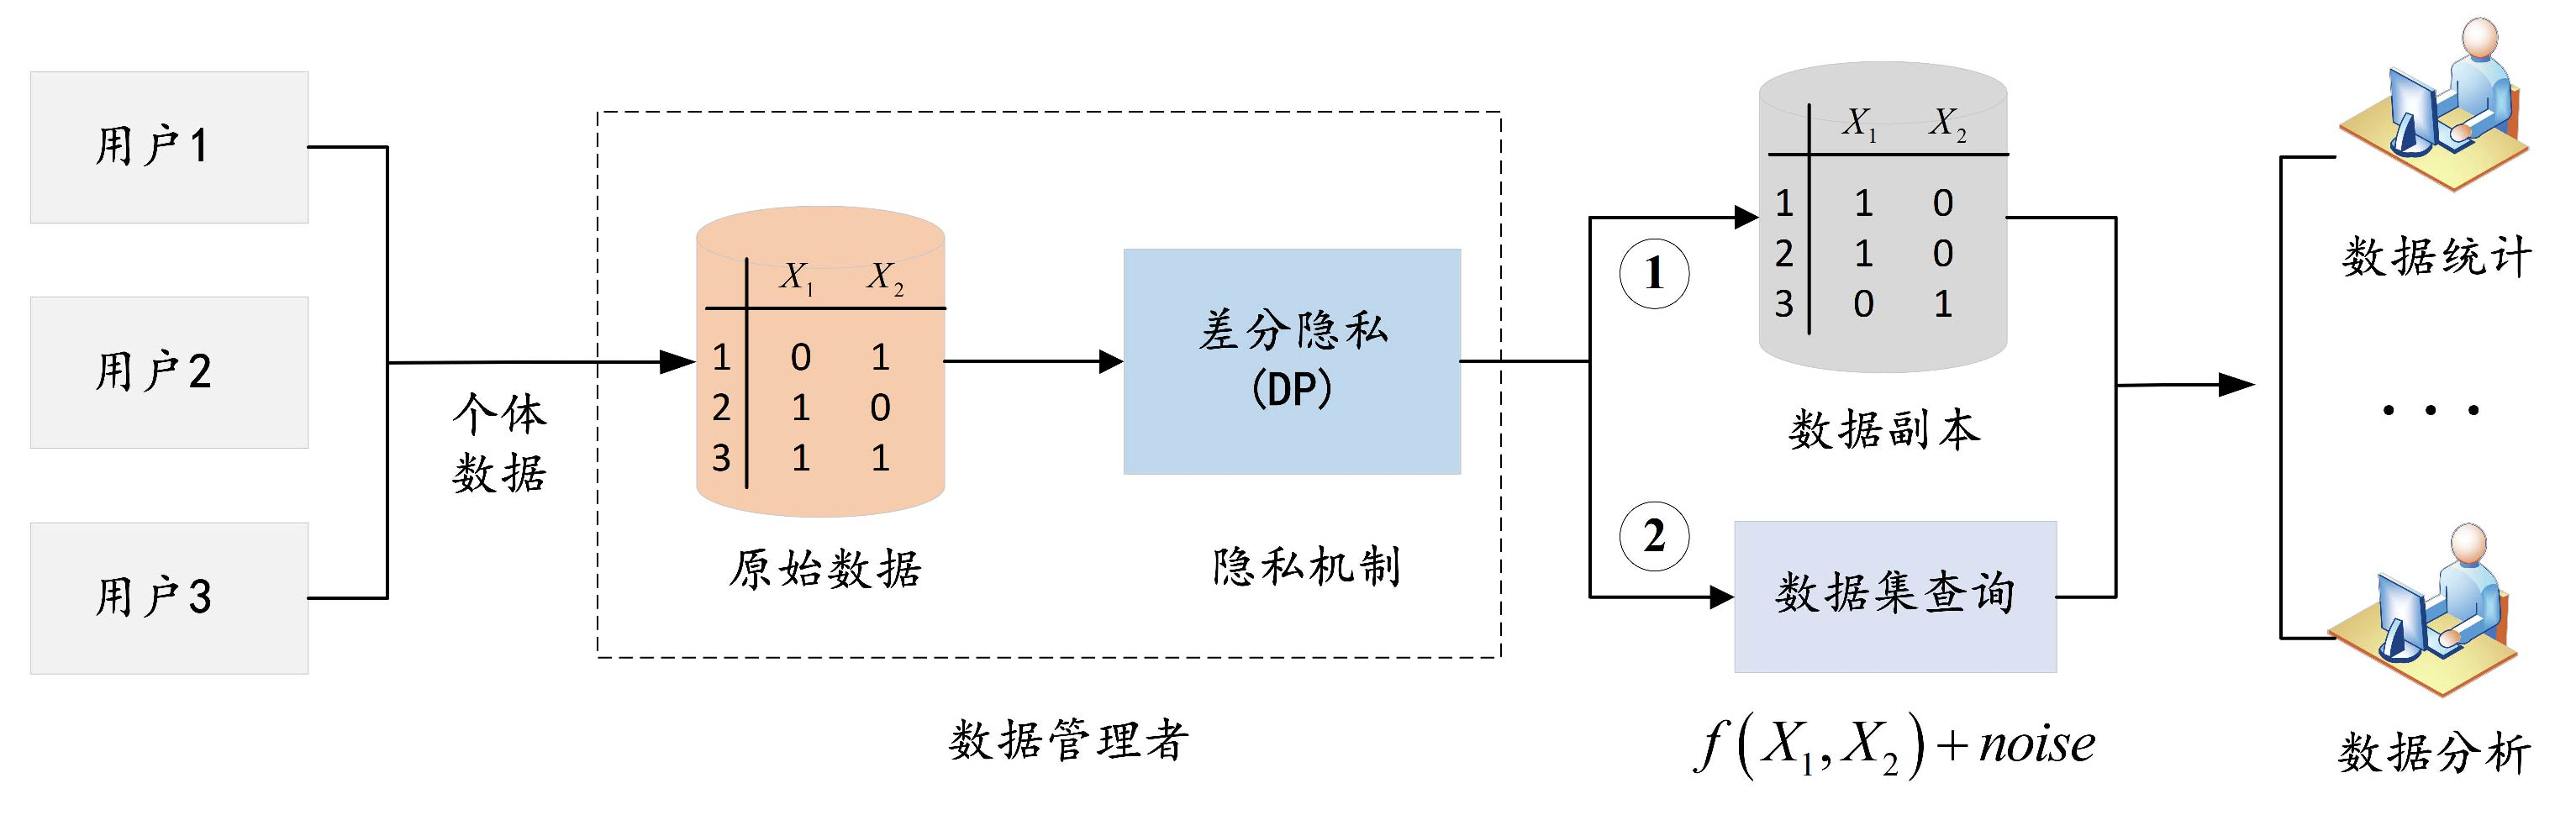
\includegraphics[width = 0.85\linewidth]{./figures/chapter02_1.jpg}
	\caption{中心化差分隐私的系统架构}
	\label{fig:chapter02-dp-model}
\end{figure}

首先,差分隐私的非交互式工作模式中,数据管理者旨在利用差分隐私机制发布原始数据集的噪声副本以供数据分析者使用(图\ref{fig:chapter02-dp-model}第$1$ 个阶段所示)。如示例\ref{example:01}中发布原始表\ref{tab:origin}的扰动数据净化副本。针对此情景,混淆产生的数据副本与原始数据之间存在着相互依存的隐私与效用平衡问题。其次,在交互式查询的数据发布场景中,对于一个查询函数$f$,差分隐私算法在查询精确的结果上增加满足特定分布的噪声,返回噪声的查询结果(图\ref{fig:chapter02-dp-model}第$2$ 个阶段所示)。交互式工作模式中,数据分析者通过查询接口提交查询请求,接收差分隐私返回的噪声结果,观察不到数据集的全貌特征。如查询婚姻状态为Separated的计数查询,则可能得到噪声结果$1.5$而不是真实的结果$1$。近年来,差分隐私的两种工作模式均得到了不同程度的应用研究,下文中我们结合具体的应用场景分析其研究发展状况。


\subsection{本地化模型}
差分隐私的实际应用中并不总是存在可信数据管理者,针对非可信管理者的系统应用中,研究者提出了本地化隐私\cite{kasiviswanathan2011what}(Local privacy)的概念,并给出了正式的定义,即是差分隐私的本地化模型\cite{duchi2013local,duchi2013Minimax}。本地化模型大多应用在隐私保护的数据收集场景\cite{wang2019collecting,fanti2016building,erlingsson2014rappor,wang2016using},在数据发布中也有部分的应用\cite{yang2017copula,ren2018textsf}。一个通用的本地化差分隐私的系统架构模型如图\ref{fig:chapter02-LDP-model}所示。
\begin{figure}[htbp]
	\centering
	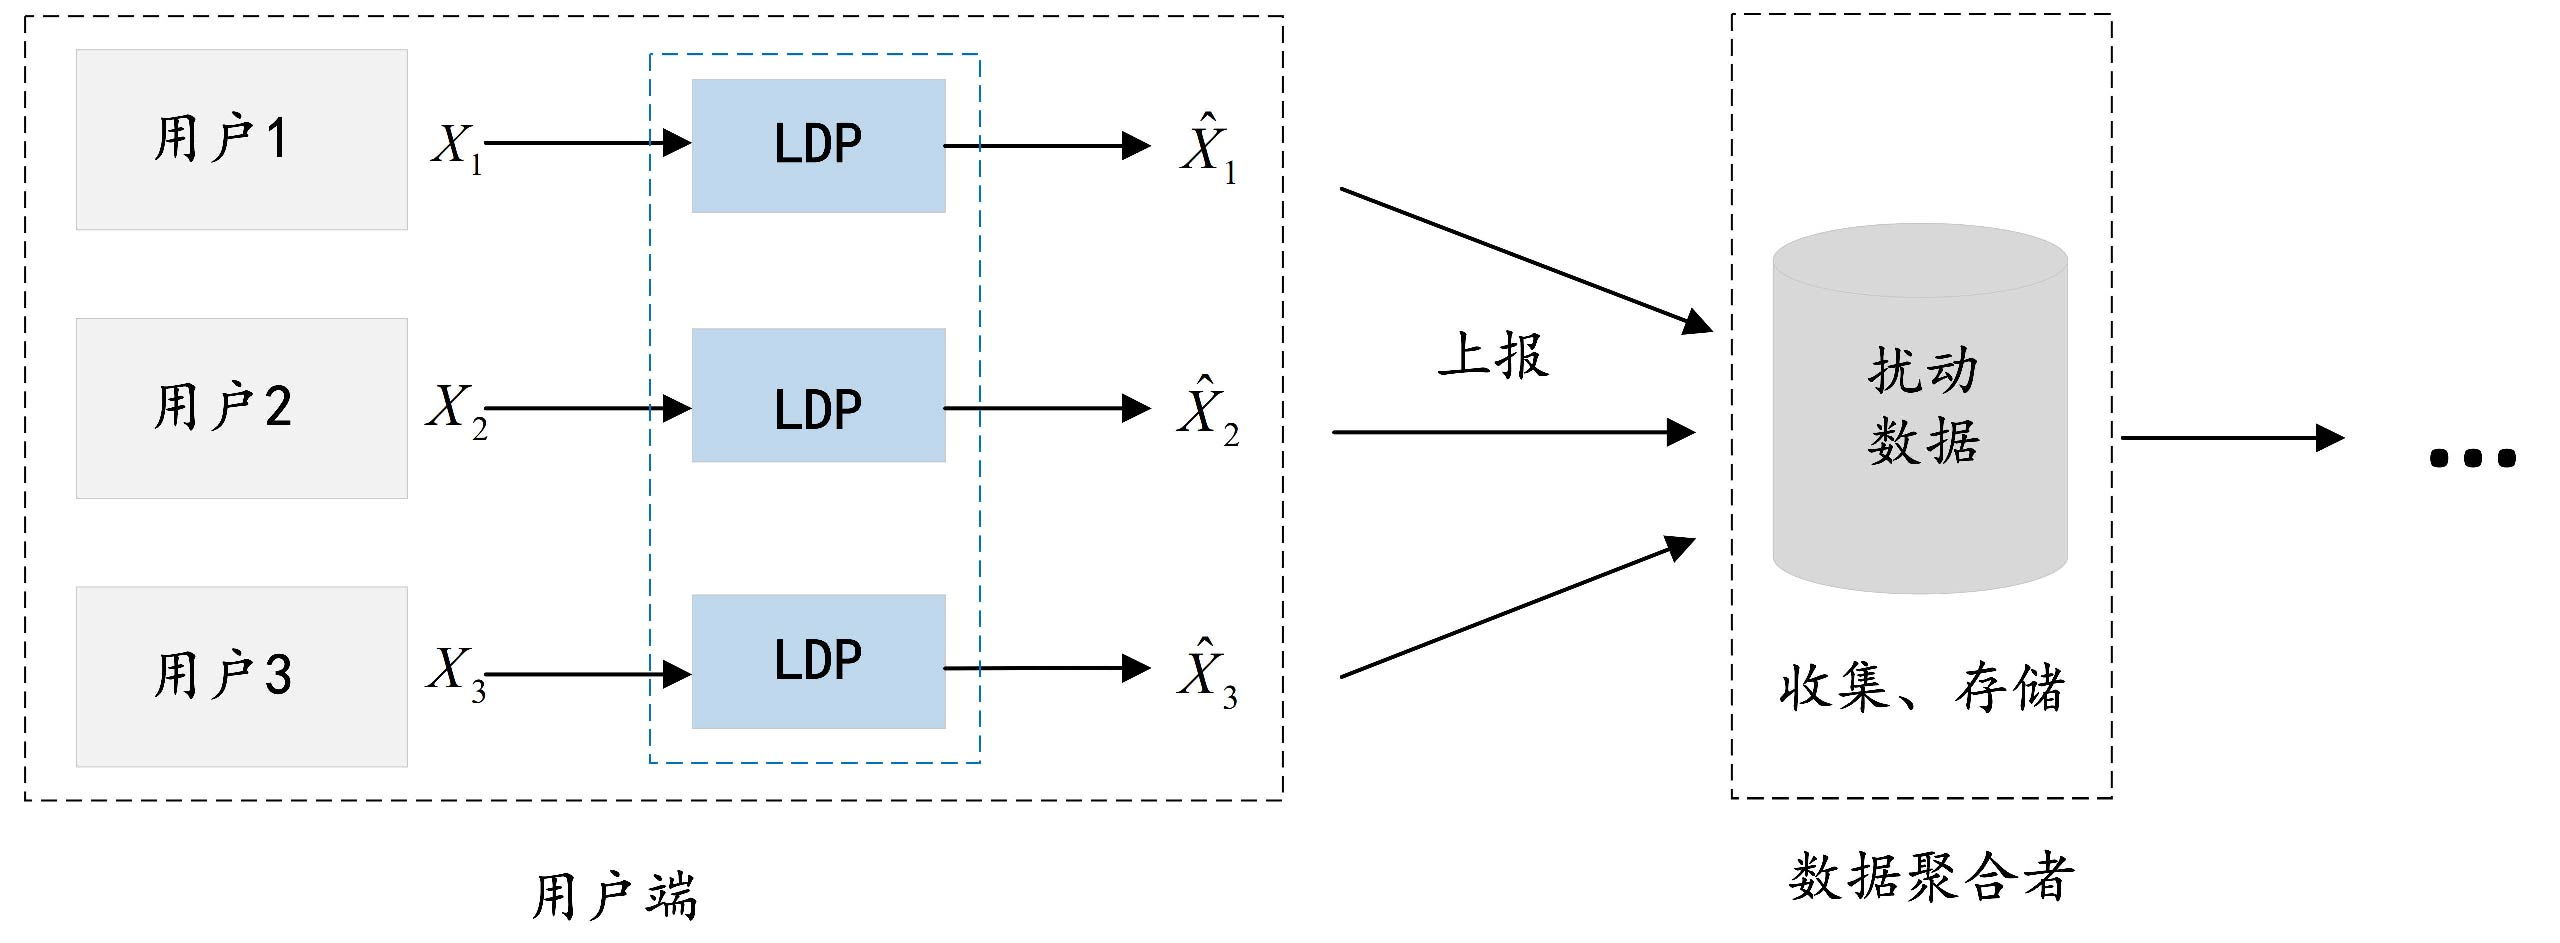
\includegraphics[width = 0.85\linewidth]{./figures/chapter02_2.jpg}
	\caption{本地化差分隐私的系统架构}
	\label{fig:chapter02-LDP-model}
\end{figure}

差分隐私本地化模型的一般应用架构中主要包括有系统用户、差分隐私机制、数据聚合者。本地模型的应用中,每一个系统用户独立的执行差分隐私算法,本地随机扰动其真实的数据信息,然后得到扰动后的数据,并将扰动后生成的伪装数据上报给数据聚合者,随后,数据聚合者收集、存储、分析这些上报的数据。近些年来,本地化差分隐私受到广泛关注。围绕本地化差分隐私的应用,研究者基于随机响应技术(RR)\cite{warner1965randomized}提出了一系列的本地化差分隐私模型与算法。接下来,我们综述近些年差分隐私应用研究中的主要成果,进一步分析差分隐私研究的发展趋势。





\subsection{差分隐私应用研究}
差分隐私现已成为隐私保护研究的标准,对其应用的研究涉及社交网络\cite{wei2020asgldp,kasiviswanathan2013analyzing}、推荐服务\cite{xiao2020deep}、移动众包计算\cite{sei2017differential}等领域,%隐私保护的数据类型从关系数据延申至图数据、键-值型数据、地理数据等不同数据类别。
图\ref{fig:chapter02-application-research}描绘了差分隐私的主要应用领域和具体场景中的核心研究问题。
本文中,围绕个人数据生命周期阶段,结合差分隐私的具体应用场景,{\em 从隐私保护的数据发布、隐私保护的数据收集、隐私保护的数据分析}角度介绍目前学术研究的现状。%随后,本文分析了在差分隐私的应用研究中需要关注的关键问题。
\begin{figure}[htbp]
	\centering
	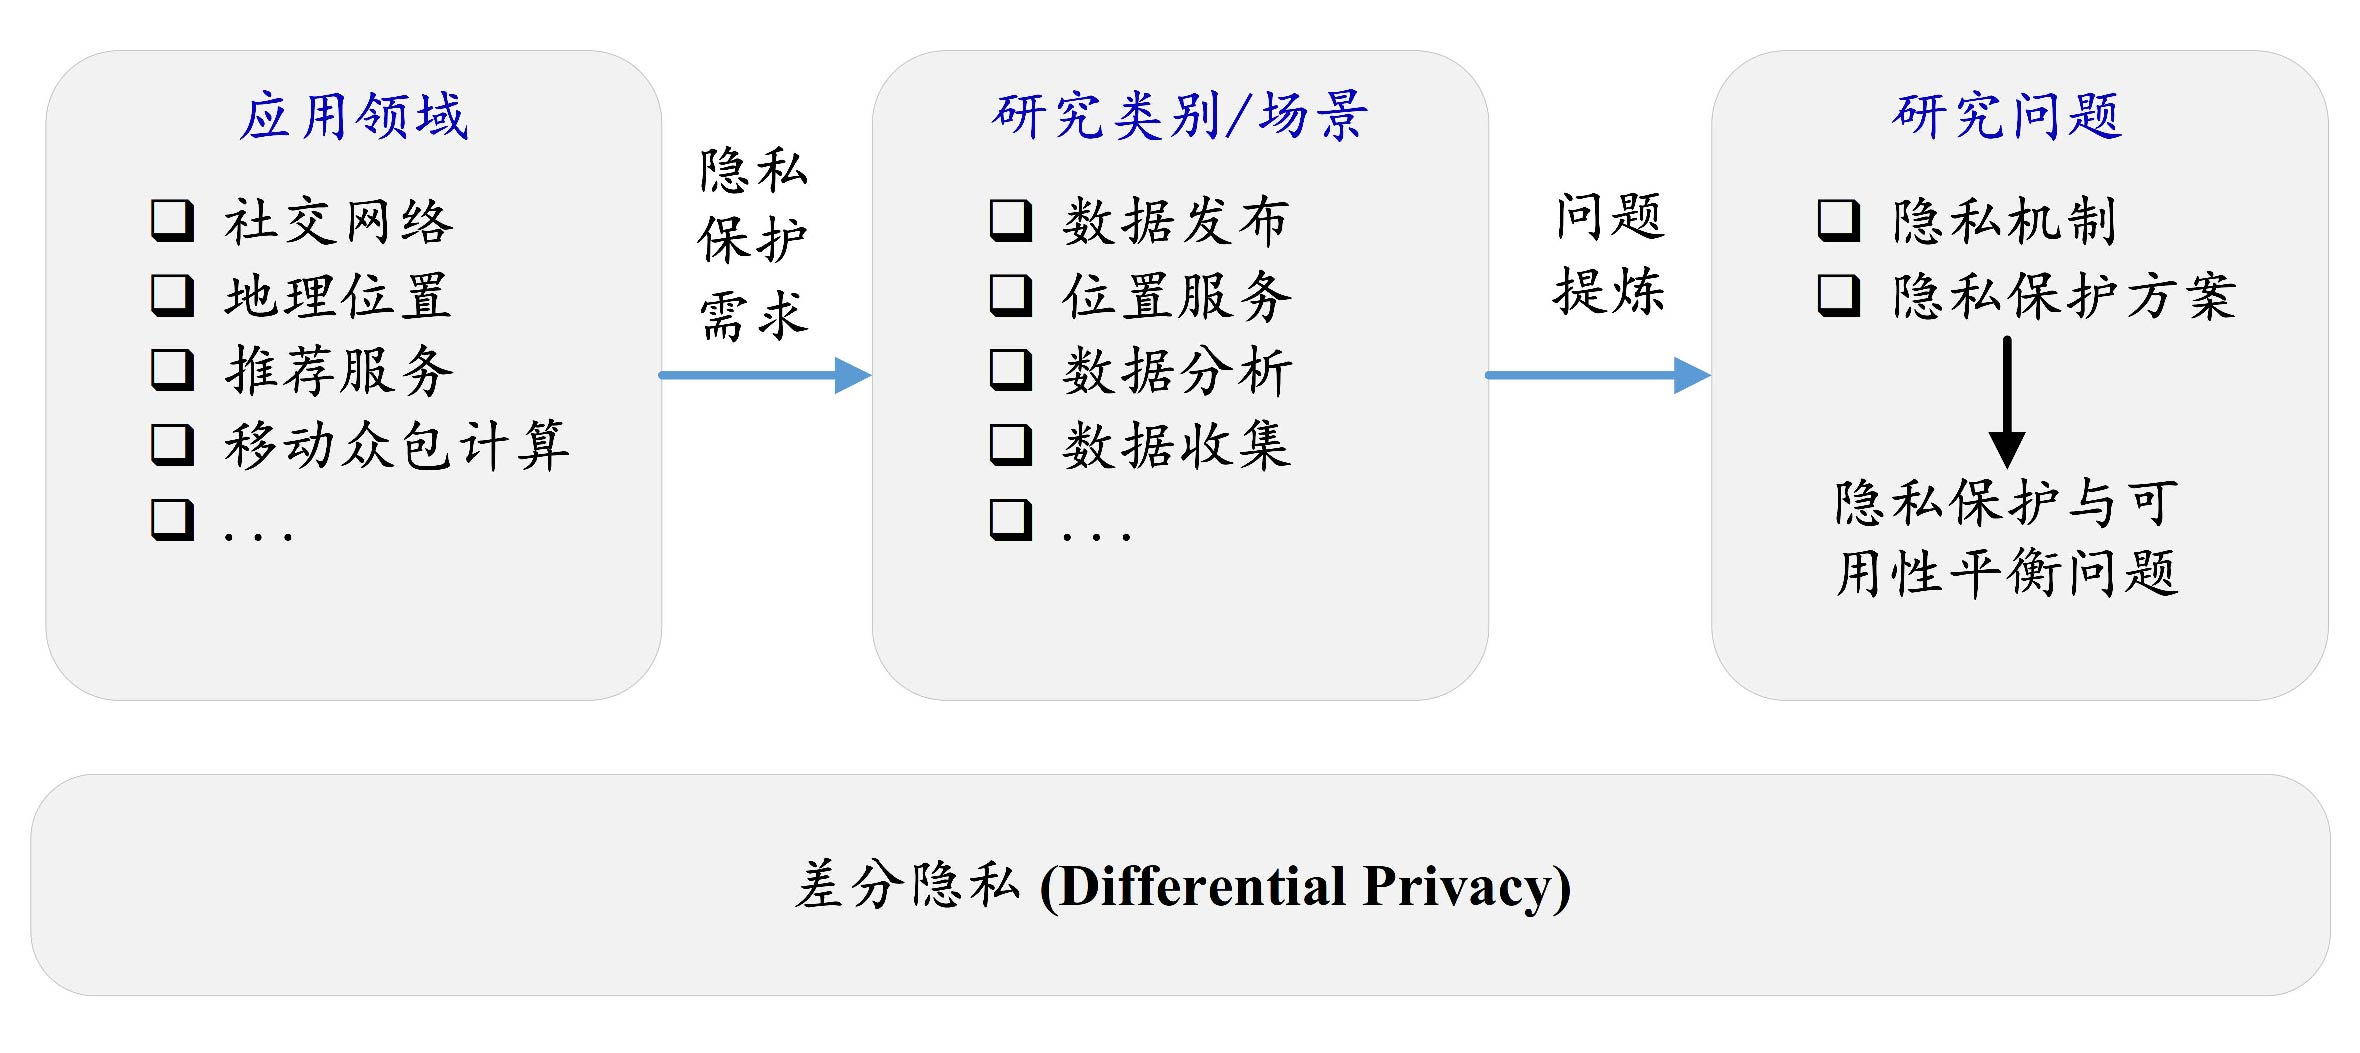
\includegraphics[width = 0.85\linewidth]{./figures/chapter02_3.jpg}
	\caption{差分隐私的应用研究}
	\label{fig:chapter02-application-research}
\end{figure}

首先,隐私保护的数据发布场景中,可信数据管理者发布数据以供进一步的数据分析\cite{aggarwal2008privacy},目标是发布数据的聚合信息而不泄露用户的个体隐私。差分隐私的数据发布包含有交互式发布和非交互式发布两种类型,其中,交互式数据发布包含有事务型数据发布、直方图数据发布、流数据发布、图数据发布;非交互式数据发布主要有批量查询发布、合成数据集发布\cite{zhu2017differentially}。隐私保护的数据发布场景中,发布数据的精确度与隐私泄露权衡是主要关注的核心问题。{\em 为了解决数据发布中存在的隐私泄露问题,差分隐私的机制是研究的核心关注点}。近年来,以Dwork的方法
\cite{dwork2006calibrating}为基础,针对不同的发布数据类型,研究者提出了诸多的差分隐私数据发布模型及算法。
表\ref{tab:survey_dp_publishing}列出了差分隐私数据发布的主要部分研究工作。




\begin{table}[htbp]
\caption{{\em 差分隐私的数据发布方法}}
\label{tab:survey_dp_publishing}
\centering
\fontsize{10pt}{\baselineskip}\selectfont
\begin{tabular}{p{0.10\textwidth}p{0.05\textwidth}p{0.30\textwidth}p{0.30\textwidth}}
\toprule
	\textbf{工作模式}& &\textbf{数据发布类型}&\textbf{主要研究}\\
	\midrule
   交互式数据发布& &\makecell[l]{事务型数据发布 \\ 直方图数据发布 \\ 流数据发布\\ 图数据发布} &\makecell[l]{
IDC\cite{gupta2012iterative}\\Laplace\cite{dwork2006calibrating},Partitioning\cite{chen2011publishing}\\ Pan-Privacy\cite{dwork2010differential},P-Sums\cite{chan2011private}\\ Edge DP\cite{zhang2015private}, Node DP\cite{kasiviswanathan2013analyzing}} \\
   \midrule
非交互式数据发布& &\makecell[l]{批量查询发布\\ 合成数据集发布} & \makecell[l]{Batch Query\cite{yuan2012low}\\ Sanitization\cite{dwork2009on}}\\

  \bottomrule
\end{tabular}
\end{table}

其次,本地化差分隐私的应用研究\cite{yeqingqing2018}已逐渐成为差分隐私的另一个重要研究分支,在隐私保护的数据收集、数据发布场景中都得到了不同程度的应用。围绕本地化差分隐私的应用,主要是研究如何设计可获得的隐私机制实现预期的目标。随机化响应技术是本地化差分隐私算法实现的基本构建模块,它在本地差分隐私中的应用取得了显著的效果。近年来,研究者提出诸多先进的本地化差分隐私方案。2014 年,Erlingsson~等\cite{erlingsson2014rappor}提出了随机聚合的隐私保护顺序响应算法(RAPPOR),该算法利用哈希函数和布隆过滤器(Bloom Filter) 将用户的真实数据~$v$~ 转换为一个长度为~$k$~的比特数组,然后基于随机响应机制(RR)对每一个比特进行随机响应,然后得到扰动的数据。但是,RAPPOR中存在着隐私变量单一、对已知数据字典的随机响应问题。为了解决这个问题,2016年,Fanti等\cite{fanti2016building}将RAPPOR扩展到更复杂没有统计背景知识的情形,提出了一种新型的算法,该算法可以实现收集单个或多个变量数据。随后,Kairouz等\cite{kairouz2016discrete} 将哈希应用到~$k$-RR和RAPPOR中,提出了O-RR~ 和~O-RAPPOR机制。周异辉等\cite{zhouyihui2019}针对隐私-效用均衡问题,从优化理论的角度给出了效用优化模型,并分析了随机响应机制的最优性条件和相应的效用最优机制。此外,对于其它数据结构的本地化差分隐私也得到了研究,如set-value的本地化差分隐私
\cite{wang2018privset,qin2016heavy}、key-value类型数据的本地化差分隐私\cite{ye2019privkv} 以及图数据结构的本地化差分隐私\cite{wei2020asgldp}。本地化差分隐私的应用涉及到社交网络\cite{qin2017generating}、移动众包计算\cite{sei2017differential}、数据合成发布\cite{ren2018textsf,yang2017copula}等场景,也因此日渐受到关注。

%此外,基于图的隐私保护数据发布\cite{li2016graph}、、 基于矩阵值查询的\cite{chanyaswad2018mvg}、

最后,隐私保护的数据分析是在保持数据分析的精确度的同时保护个体的隐私信息\cite{wang2016on}。近年来,基于学习理论(learning theory)的方法在差分隐私中得到了具体的应用,包括数据分析与机器学习的方法在差分隐私中的应用\cite{kasiviswanathan2011what,ye2017optimal,sarwate2013signal}(如概率分布估计\cite{Murakami2018Toward},数据训练\cite{xu2019ganobfuscator})。2018年,Ren 等\cite{ren2018textsf} 使用~EM~和~Lasso~的方法进行分布估计,用于得到联合概率分布,支撑新的数据集合成。2019年,Wang等\cite{wang2019collecting}基于机器学习的线性回归(linear regression)、逻辑回归(logistic regression)、支持向量机(support vector machines, SVM)分类算法分析了所提出分段机制(piecewise mechanism,PM)和混合机制(hybrid mechanism,HM)的性能。由此可知,隐私保护的数据分析主要是学习数据的统计特征,体现出扰动数据的质量。

%综上所述,差分隐私在隐私保护中占据着重要的地位,它已经涉及到了具有隐私保护需求的各种信息系统应用。现阶段,差分隐私在面向低维数据和独立同分布数据情景的研究相对比较成熟,具有一系列较为成熟的研究方案。但是,随着应用系统的需求升级,在面向多维或高维数据且存在数据关联的情景时,差分隐私机制将面临新的挑战。针对此,研究者进行了积极的探索,以下给出研究进展及现状的介绍。

鉴于上述的分析可知,差分隐私在隐私保护的研究中占据着重要的地位,它已经涉及到了具有隐私保护需求的各种信息系统应用。现阶段,差分隐私在面向低维数据和独立同分布数据情景的研究相对比较成熟,具有一系列较为成熟的研究方案。但是,随着应用系统的需求升级,在面向多维或高维数据且存在数据关联的情景时,差分隐私机制将面临新的挑战。针对此,研究者开展了积极的探索研究工作,以下给出研究进展及现状的介绍。

\section{差分隐私研究动态}
大数据环境下,原始数据的结构特征给差分隐私数据处理带来新的挑战,亟待研究者深入研究提出新的差分隐私模型及算法。具体来说,多维数据或高维数据、数据关联以及用户个性化的隐私偏好等原因带来的研究新课题。本节中,围绕这些问题的解决方法,介绍差分隐私的学术研究动态。

\subsection{面向多维数据的差分隐私}

随着用户数据维度的增加,多维或高维数据具有笛卡尔乘积空间大、数据稀疏性的特点,给差分隐私数据处理带来新的挑战。具体地说,差分隐私对于多维数据或高维数据的处理主要面临着隐私脆弱性、计算复杂度高等问题。为了解决这些问题,数据降维是一种通常采用的处理方法。将有关个体的数据元组,拆分为多个属性分量,然后独立的应用差分隐私机制,该处理思想以差分隐私的并行组合原理为基础,其基本的处理流程可以表述为图\ref{fig:chapter02-multidimension-data}所示。

\begin{figure}[htbp]
	\centering
	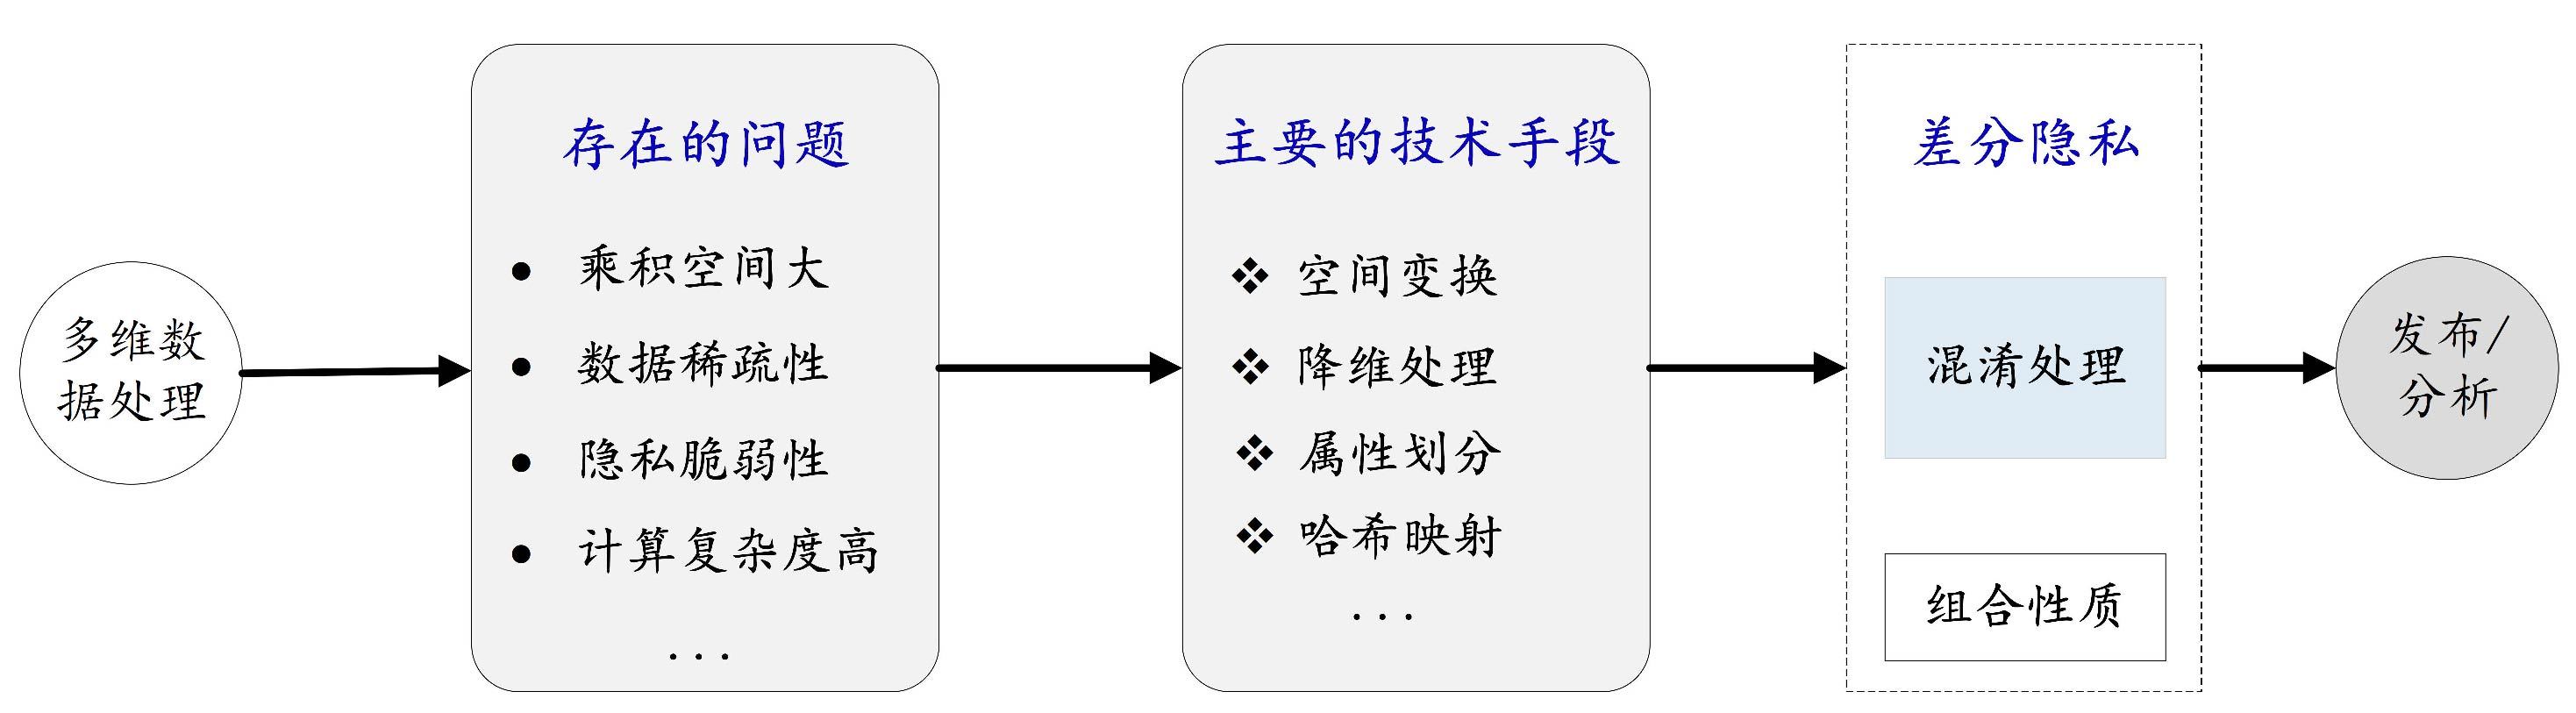
\includegraphics[width = 0.85\linewidth]{./figures/chapter02_4.jpg}
	\caption{差分隐私的多维数据处理流程}
	\label{fig:chapter02-multidimension-data}
\end{figure}

针对差分隐私的多维数据处理,研究者做了一些有意义的探索,提出了差分隐私的多维数据处理方案。2017年,Xu等\cite{xu2017dppro}针对多维数据发布中存在的扰动误差增加和计算复杂性问题,通过随机投影的方法提出了高维数据发布的DPPro方案。此外,在本地化差分隐私模型中,Wang等\cite{wang2019collecting}推广并改进了Duchi等人\cite{duchi2018minimax}的方法,针对多维数据的收集和分析提出了分段机制和混合机制,其思想是将属性分为类别型和数值型属性,然后依赖于单一数值型扰动方案和类别型扰动方案(optimized local hashing,OLH),实现多维混合数值型和类别型数据的处理。Ren等\cite{ren2018textsf}拓展低维数据处理的RAPPOR到高维数据情景,利用属性值拆分、扰动合并和差分隐私的组合定理\cite{kairouz2017the},考虑了差分隐私高维数据收集和发布的问题。其基本思想是将元组进行属性拆分,然后利用哈希函数和布隆过滤器映射属性值到比特串,并逐比特的进行随机扰动,产生扰动的元组。如表\ref{tab:origin}原始数据,该方法首先哈希得到``0''和``1''的比特串,然后随机响应,最后实现随机扰动。此外,Yang等\cite{yang2017copula}基于随机响应技术本地转化用户数据到比特串,实现多维数据合成和发布的机制。事实证明这是一种相对有效的处理方法,且被广泛的应用在隐私保护的多维数据情景。该思想在基于地理位置的隐私保护系统中也有相应的应用,如混淆扰动一个元组时,独立的应用存在的隐私保护机制到元组的每一个位置点,然后得到整个响应的混淆元组\cite{andres2013geo}。近年来,面向多维数据的差分隐私研究逐渐成为一个重要的研究点,但是,目前针对混合数值型和类别型的多维属性的差分隐私最优化机制的研究还相对较少,尚需要进一步的研究。

%差分隐私根据是否存在可信的第三方数据管理者可以分为中心化差分隐私和本地化差分隐私。通常情况下并不存在可信的第三方数据管理者。因鉴于此,本地化差分隐私在隐私保护的数据收集、发布场景得到了广泛研究。最早,可追溯到1965 年Warner\cite{warner1965randomized}为解决统计数据库存在的个体隐私泄露问题,提出随机化响应(RR)机制。此后,针对无可信数据管理者的隐私保护数据收集场景,开展了一系列的研究工作。2016 年,Wang等\cite{wang2016using} 研究了二进制属性的随机响应机制效用最优化,并进其推广到多属性的随机响应(MRR) 机制。同年,kairouz等\cite{kairouz2016extremal}提出了针对类别型属性的$k$-RR响应机制,随机映射到任意可能数量的响应值。此外,在隐私保护的数据收集场景中的隐私效用最优化方面,研究了差分隐私的最优化随机响应机制问题。2017 年,Holohan等\cite{holohan2017optimal}基于Warner的随机化响应(RR)技术,在差分隐私约束条件下,研究了二元单属性随机响应的最优化机制问题,给出了$\epsilon$-差分隐私最小估计误差的设计矩阵形式,该矩阵拥有对称矩阵的形式。叶青青等\cite{ye2019privkv,yeqingqing2018}针对key-value 型数据研究了隐私保护数据收集场景中的本地化差分隐私随机化响应机制。此外的一些研究工作推广二元随机响应到多元随机响应旨在收集、发布高维\cite{yang2017copula}。2018年,Ren等\cite{ren2018textsf}在Bloom Filter和随机化响应机制(RR) 的基础上,利用属性值拆分、扰动合并和差分隐私的组合定理\cite{kairouz2017the},考虑了差分隐私高维数据收集和发布的问题。由此可知,目前针对混合数值型和类别型的多维属性的多元随机化响应(MRR)的最优化机制的研究还较小,且是一个有意义的探索研究方向。


\subsection{面向数据关联的差分隐私}

现有的方法大多假设数据抽样独立,然而实际应用中,多维数据通常不是独立存在,而是存在着关联的情况。这些关联可以分为数据的记录关联、属性关联或隐私攻击者的关联辅助背景知识关联等情况。文献\cite{kifer2011no}揭示了相关数据上的隐私机制将比期望的泄露更多的信息。近些年,数据关联的差分隐私受到研究者关注。

{\em 表\ref{tab:origin}所示的数据信息中,属性Age、Occupation可能和Marital-status存在属性关联,这种关联使得敌手能够以较高的置信推断用户的隐私信息,从而增加隐私泄露风险。例如,文献\cite{zhu2015correlated}揭示由属性导致的元组相关,增加了流感疾病隐私泄露风险;文献\cite{li2019impact}分析了敌手背景知识对隐私泄露的影响。}针对数据关联的隐私泄露影响,研究者开展了相关的研究工作。
2014年,Zhang 等\cite{zhang2014privbayes}利用贝叶斯网络考虑了数据集属性关联的情景,借助互信息分析属性之间的相关度\cite{reshef2011detecting,liangjy2016},提出利用贝叶斯网络实现差分隐私的高维数据发布。2015年,Zhu等\cite{zhu2015correlated}针对非独立同分布的数据集记录关联,改进了差分隐私的敏感度计算方法,减少了噪声注入提升了数据效用。Yang等\cite{yang2015bayesian}研究了数据相关对隐私的影响,敌手先验知识对隐私的影响和数据相关时的扰动算法设计,提出了贝叶斯差分隐私。2017年,Song等\cite{song2017pufferfish}提出Pufferfish privacy保护关联数据的隐私。2019 年,Li 等\cite{li2019impact} 基于皮尔逊的相关度分析方法,从强关联、弱关联、正相关和负相关的角度,考虑了隐私攻击者的背景知识和数据关联对差分隐私数据发布的影响。鉴于上述分析,由数据的记录关联、属性关联或隐私攻击者的关联辅助背景知识,导致的隐私泄露问题,或是存在数据关联的高维数据发布问题仍然是学术研究关注的焦点。数据相关的隐私度量分析成为隐私机制设计首要解决的问题。


%Dwork的方法首先映射记录到一个频率矩阵,添加独立噪声在频率矩阵的每一记录,发布噪声频率矩阵\cite{dwork2006calibrating}。该方法对于大量记录的聚合查询,近似查询结果有$O(m)$噪声方差。实际中,数据集通常包含多个属性,以至于域值很大,导致此方法引入过大的噪声量。如文献\cite{xiao2011differential} 利用小波变换减少注入噪声。此外,数据集通常存在关联,数据关联引发差分隐私噪声与效用问题。
\subsection{面向用户偏好的差分隐私}

差分隐私模型扩展应用于多维数据时,差分隐私的隐私特性($\epsilon$-度量)由其组合性质保障。通常情况下,差分隐私把多维属性看作等价敏感,提供相同等级的隐私保护。例如,用户个体的隐私数据包含$d$个属性维度,差分隐私机制的隐私预算设置$\epsilon/k$,然后依据序列组合性质,隐私保护总体满足$\epsilon$- 差分隐私。但是,多维的属性之间可能存在不同的隐私敏感度,也就是用户的隐私敏感偏好。为了更好的阐述这个问题,首先给出以下问题引例。

{\em 假设个体数据元组由年龄、性别、教育程度、婚姻状态组成,这些数据项都是有关个体的隐私信息。但是,在这些数据项中,用户对其数据具有不同的隐私感受。通常情况下,一个人的性别可能不被认为是隐私数据或者具有较低的隐私敏感性。然而,一个人的婚姻状态(如离婚)是想保持私密性的敏感数据,其隐私私密性高于其它属性。}为了能够解决诸如此类的问题,这就要求差分隐私能够提供不同敏感等级的隐私保护对于有区分的属性,满足所提出的隐私保护需求。

针对上述问题,研究者依据属性敏感度等级,提出了有区别隐私数据的个性化差分隐私保护方案\cite{chen2016private}。2015年,Jorgensen等\cite{jorgensen2015conservative}考虑个人数据的不同隐私保护需求,提出了个性化差分隐私(personalized differential privacy, PDP)的概念。2019 年,Wang等\cite{wang2019personalized}利用泛化的$d_{\mathcal{X}}$-privacy\cite{chatzikokolakis2013broadening}研究了个性化隐私保护。Murakami 等\cite{murakami2019utility} 提出了效用最优的本地化差分隐私方案(Utility-optimized LDP,ULDP)用于隐私保护的数据收集与分析。通过划分个体数据为敏感数据和非敏感数据两部分,推广Mangat\cite{mangat1994an}随机响应到多元字母表情景,提出了ULDP方案,对于敏感的数据提供和LDP 等价的隐私保障。2020年,Gu 等\cite{gu2020providing}通过考虑不同输入数据具有不同的隐私敏感度,提出了一种输入区分(input-discriminiative)的隐私保护机制ID-LDP。由此可见,考虑用户隐私偏好,设计差分隐私机制,实现为不同敏感度的用户数据提供有区分的隐私保护成为一种新的研究方向。

\section{差分隐私研究趋势}
Shannon\cite{shannon1948a}为解决信息度量问题提出信息熵的概念之后,信息熵在通信、密码学等领域发挥了重要的作用。近年来,基于信息度量的量化信息流思想(quantitative information flow, QIF)逐渐在隐私保护中得到应用。此外,博弈均衡理论作为一种有效的分析工具在隐私保护中也得到了应用。针对差分隐私应用中存在的隐私与效用的平衡问题,基于信息论、博弈论以及交叉学科的方法开展研究逐渐成为新的研究方向。以下从两个方面综述密切相关且具有代表性的研究成果。

\subsection{差分隐私的信息论方法}\label{subsec:information_dp}
隐私保护模型的本质是混淆、扰动机制,它可以表达为一种概率性的函数映射,与信息论的方法密切相关\cite{Duchi2019information}。由此,在隐私保护研究中,信息熵发展成为一种有效的隐私度量方法\cite{issa2016an,Chatzikokolakis2008Anonymity}。以信息熵为基础定义的R\'{e}nyi熵\cite{renyi1961on,erven2014renyi,mironov2017renyi}、条件熵、联合熵、互信息量等在隐私保护研究中得到了应用\cite{wang2019consistent,mcgregor2010the,du2015Fundamental,lopuhaa-zwakenberg2019information}。隐私度量方面,Mir 等\cite{mir2012information}利用条件熵、互信息量研究了隐私信息的度量问题,奠定了差分隐私的信息论方法研究基础。Barthe 等\cite{barthe2011information} 利用信息熵研究了差分隐私的隐私边界问题。Issa等\cite{issa2016an,2016Maximal}Maximal leakage测量隐私泄露,随后,Liao等\cite{liao2019tunable}对其扩展提出$\alpha$-leakage。其次,信息论的方法对于差分隐私的机制研究也有一定的应用\cite{diaz2020on,kairouz2016extremal,wang2016on}。2011年,Alvim 等\cite{alvim2011differential,alvim2011on,alvim2015on}几乎是最早提出基于量化信息流(QIF) 的思想,将信息熵应用到差分隐私中量化隐私信息的不确定度,抽象差分隐私噪声机制为信息论噪声信道,并从信息论的角度考虑了平衡隐私度与数据效用的方法,同时提出信息论对称信道机制能够达到理论最优性。随后,信息论方法研究的差分隐私与标准差分隐私的关系得到研究者的关注\cite{mcgregor2010the}。Cuff 等\cite{cuff2016differential}基于互信息的概念给出了与标准差分隐私等价的信息论差分隐私定义。文献\cite{calmon2012privacy,makhdoumi2013privacy}研究建立了互信息约束与差分隐私的关系。进一步,Wang 等\cite{wang2016on}提出可辨识识别(identifiability)的概念、并研究了与差分隐私(differential privacy) 和互信息隐私(mutual information privacy) 三个不同隐私概念之间的基本联系。更重要地是,信息论中著名地信源编码定理、限失真编码定理(保真度准则)\cite{cover2006elements}在隐私保护中均得到了相应地研究\cite{rebollo-monedero2010from,du2015Fundamental}。如Sankar等\cite{sankar2013utility}针对统计数据库隐私泄露问题,构建了统计数据库的概率模型,从最佳信源编码、译码方案的角度考虑了信息论方法在数据库隐私与效用平衡中的应用。允许部分失真情况下,最小信息传输率的率失真理论在差分隐私\cite{mir2012information,wang2016on}最优机制研究中也受到了关注。

随机响应技术是实现本地化差分隐私的有效方法,信息论方法对于随机响应的研究也得到了广泛的应用。事实上,本地化差分隐私的随机响应实现是根据特定的概率密度函数(probability density function, PDF)随机响应。在此方面的研究关键在于设计满足差分隐私的概率密度函数。近年来,信息论方法的研究已从二元随机响应逐步发展到多元随机响应,逐步向复杂数据类型拓展延申。具体研究工作从信息论的本地化差分隐私度量
\cite{lopuhaa-zwakenberg2019information},向最优机制设计发展。Sarwate 等\cite{sarwate2014a}抽象二元离散随机响应机制为Shannon 信息论\cite{shannon1948a}离散噪声信道,基于率失真理论\cite{cover2006elements} 对本地化差分隐私的二元随机响应机制进行了研究,指出对称信道机制能达到最优性。二元随机响应仅能处理`` 是''和``否''的问题,其应用具有局限性。随后,研究者对其进行了拓展研究,发展了多元随机响应(multivariate random response, MRR) 技术。Kairouz等\cite{kairouz2016extremal} 基于互信息提出了$k$-RR机制,并在此后被进一步研究,发展了一系列先进的隐私机制。Kalantari 等\cite{kalantari2018robust}考虑不同先验概率分布情况,研究了汉明失真下平衡隐私度与数据效用的最佳差分隐私信道机制问题,指出对称信道机制和非对称信道机制的最优性对不同分布的最优性。Xiong 等\cite{xiong2016randomized}在隐私保护的数据收集场景,利用信息论的方法,将差分隐私的数据扰动机制抽象为离散无记忆的噪声信道机制,从限失真约束条件定义差分隐私信道集合,研究了本地化差分隐私的机制问题。

{\em 基于这些相关的研究工作,可以看出信息论的方法应用于差分隐私研究,主要是解决两个方面的问题:(1) 隐私信息的度量问题;(2) 差分隐私的机制设计问题。}首先,前者的研究主要是从熵的内涵角度理解隐私泄露问题,该研究可用于评估隐私泄露风险(例如,定量分析隐私泄露的界),同时也是信息论方法对差分隐私机制研究的基础;其次,为了解决隐私与效用的平衡问题,后者的研究主要关注于最优的差分隐私实现机制。对于该问题的解决,信息论方法是从噪声信道角度寻找满足给定约束条件的最优条件概率分布。由此,基于优化理论建模\cite{iyengar2019towards}、求解该问题是一种理想的选择。如极大极小定理、Karush-Kuhn-Tucker (KKT)条件等\cite{boyd2004convex}得到了具体的应用。结合凸性或拟凸性形式化隐私与效用平衡问题为拟凸优化问题\cite{xiong2016randomized}、隐私失真最优化问题\cite{wang2016on}(信息论领域的率失真问题)
是较好的解决方法。但是,现阶段信息论方法总是假设数据抽样独立,对多维数据情景、多维属性存在关联、混合数值型和类别型的最优差分隐私机制问题尚未充分研究。


%并将隐私数据压缩效用平衡形式化表述为基于离线无记忆信道的拟凸优化问题。
%
%kalantari 等\cite{kalantari2016optimal}针对结构化的信源数据考虑了汉明失真度量下的差分隐私最优化机制问题。此后,此外,互信息最优性离散隐私数据分布估计\cite{wang2016mutual,wang2019local}、极大极小率的估计
%\cite{duchi2013localprivacy,duchi2013local,liu2019minimax}也得到了研究和关注。鉴于此,信息熵\cite{shannon1948a}、Renyi熵
%\cite{renyi1961on,erven2014renyi}、率失真函数\cite{Shannon1959Coding,cover2006elements}等在差分隐私中度量隐私泄露、研究隐私效用平衡具有理论研究意义和实际可行性。
%
%,如同样,信息论的方法在差分隐私中的研究也得到了学者的广泛关注。此外,率失真理论在差分隐私中也得到了应用。2015年Wang 等\cite{wang2015a} 基于极小极大的失真视角考虑了差分隐私数据发布问题。2016 年,Wang等\cite{wang2014on,wang2016on}针对差分隐私非交互式数据发布场景,构建了以数据库实例为随机变量,并基于期望汉明失真从发布数据库全局层面,考虑了可辨识识别(Identifiability)、差分隐私(Differential Privacy) 和互信息隐私(Mutual Information Privacy) 三个不同隐私概念之间的基本联系,并基于失真测量建立了隐私失真最优化目标函数,给出了差分隐私信道机制最优性的KKT\cite{boyd2004convex}条件,最终从理论上证明了$\epsilon$- 互信息最佳机制满足$\epsilon$-差分隐私。


\subsection{差分隐私的博弈论方法}

隐私与效用的平衡问题(privacy-utility tradeoffs)是隐私保护数据收集、隐私保护数据发布等应用场景中广泛关注的矛盾冲突问题。直观地,隐私保护效果越好,则噪声扰动导致的数据质量损失越大,以至于数据效用降低。反之,数据效用越高,则隐私保护强度较弱,由此引发的隐私泄露量较大,这被称为隐私与效用原则\cite{sankar2013utility}。在隐私保护的模型与算法研究中,如何平衡隐私与效用是一个研究的关键问题。针对此,上述优化理论的方法是一种行之有效的解决方案。除此之外,基于最优性发展起来的博弈论\cite{Neumann1944The}也为隐私保护提供了有效的分析手段。博弈分析方法从理性的角度分析在存在矛盾冲突情景下的参与者最优策略选择问题。近年来,在差分隐私研究中得到了一定程度的应用,其基本思想是分析隐私保护系统中参与者的理性行为,以均衡的思想解决隐私保护与数据效用平衡问题。

Wu等\cite{Wu2017Game}考虑了差分隐私关联数据集发布的隐私预算参数选取问题,通过构建一个多方的有限策略型博弈,利用纳什均衡的存在性条件\cite{Glicksberg1952A} 分析判断了纯策略纳什均衡存在的海塞矩阵,旨在通过纯策略的纳什均衡平衡隐私与数据效用。Hsu等\cite{Hsu2012Differential} 在差分隐私框架下针对隐私查询发布问题,建立了数据拥有者和数据查询者之间的两方零和博弈模型,提出一种新的隐私机制。Qu等\cite{cui2019improving}针对隐私与数据效用之间的权衡问题,提出了一种基于社会距离的个性化差分隐私方法,在用户和敌手之间建立了静态贝叶斯博弈,从贝叶斯纳什均衡的角度权衡隐私与效用。此外,非合作的微分博弈\cite{gao2019a}和斯坦伯格博弈(Stackelberg)\cite{fioretto2020differential} 也都在差分隐私中得到了研究。值得强调地是,Alvim 等\cite{alvim2017information,alvim2018leakage}基于量化信息流的思想,采用信息论方法度量隐私泄露,构建了隐私保护攻击与防御地两方零和博弈模型,进一步,基于极大极小理论\cite{du1995minimax}分析了隐私防护者与隐私攻击者的最佳策略选择。该研究工作将信息论的方法融入到博弈模型中标志着一种新的研究趋势。Shokri\cite{shokri2015privacy}将信息论的方法融合到博弈框架中,研究了...。但是,该研究工作没有针对具体的差分隐私保护模型研究,因此,在该方面仍然存在较大的研究提升空间。研究的关键问题在于分析具体应用场景中,隐私保护参与者和策略集,定义合理的收益函数,解决均衡的问题。


%博弈论\cite{Neumann1944The} 作为一种针对存在矛盾冲突问题有效的分析工具,自然可以引入到隐私保护模型中,分析隐私与效用的冲突,探寻纳什均衡策略平衡隐私保护与数据效用。2007年,McSherry等\cite{mcsherry2007mechanism} 在差分隐私框架下考虑了博弈的机制设计问题,旨在获得一个激励参与者真实上报隐私信息的激励相容机制。2011年,Kifer 等\cite{kifer2011no}应用`` 没有免费的午餐''定理定义一个博弈,分析差分隐私保护机制。2012 年,2013 年,Xiao 等\cite{xiao2013is}应用博弈论中真实上报机制解决数据的真实性问题。2017年,此外,由此可知,博弈论已在差分隐私中得到了应用,并且结合隐私信息量化构建隐私保护的攻防博弈,从纳什均衡的角度分析隐私与效用平衡已成为一种新的研究趋势。

\section{本章小结}

本章围绕数据开放共享、应用中存在的隐私泄露问题,首先介绍了隐私保护技术的发展,以及差分隐私提出的动机和背景。然后,针对差分隐私概述了它的应用系统架构模型及其工作模型,包括中心化模型和本地化模型。以此为基础,介绍了差分隐私的应用研究现状,重点阐述差分隐私在隐私保护的数据发布场景、数据收集以及数据分析场景中的应用研究。进一步,从多维数据、数据关联以及用户隐私偏好的角度,介绍差分隐私的学术前沿动态。最后,介绍了信息论、博弈均衡方法在差分隐私中的应用,以及现阶段针对差分隐私的学术研究发展趋势。本章中综述分析了目前的主要研究工作,明确了在差分隐私的应用中需要进一步解决的问题,为本文的后续研究工作确定了研究方向。



%
%近年来,国内的学者逐步关注信息论的方法在隐私保护领域的应用。彭长根等\cite{peng2016}借鉴Shannon 基本通信框架,结合信息论抽象隐私信息传播的基本通信模型,提出了隐私保护的基本信息熵模型、含敌手攻击的隐私信息熵模型和主观感受的加权隐私信息熵模型,并进一步提出了利用信息熵的方法度量隐私保护机制的信息泄露风险,为隐私保护效果评价提供了一种基于信息论的理论参考。此外,吴振强等
%\cite{zhenqiangwu2019} 提出了利用网络结构熵的方法度量社交网络的差分隐私保护效果。熊金波等\cite{xiongjinbo2018}从信息度量的角度综述分析了面向云计算的隐私度量。由此来看,信息论与差分隐私的结合已逐渐成为新兴的交叉研究方向,但目前国内学者针对该领域的研究处于起步状态。
%
%综合以上几个方面的研究现状,
%
%在率失真函数的求解计算方面。1959年,Shannon基于通信编码理论提出了保真度准则,即是著名的率失真理论\cite{Shannon1959Coding}。率失真函数是一个凸函数的标准最小化问题,在利用Larange乘子法求解过程中,直接解出最优输出分布是困难的。基于此,Blahut\cite{blahut1972computation} 和Arimoto\cite{arimoto1972an}提出交替最小化算法(Blahut-Arimoto) 解决率失真函数计算困难问题。Csisz\'{a}r\cite{csiszar1984information}已经证明如果集合是概率分布集合且距离度量是相对熵,则算法收敛到两个分布集合的最小熵。进一步在文献\cite{csiszar1974on}中证明了交替最小化过程中存在的极限为率失真函数$R(D)$。
%
%
%差分隐私的贝叶斯规划
%\cite{barthe2016differentially}。
%此后,Sankar研究团队的成员此外,文献。
%更多的,隐私与失真问题在基于位置的隐私保护领域也得到了研究与应用。
%2019 年,Zhang 等
%\cite{zhang2019online}在基于位置服务(Location Based Service,LBS)的隐私保护方面,基于平均互信息量和Euclidean 距离失真度量考虑了一种在线位置轨迹发布的信息论方法。该方法考虑了隐私攻击的辅助背景知识,并基于条件互信息量解决隐私与效用平衡的率失真函数最优化问题。利用一阶马尔可夫模型设计了一个在线发布的位置隐私保护机制(LPPM),获得了隐私与数据可用性的最佳权衡。Renyi\cite{renyi1961on} 熵的测量和信息的测量,同时Renyi 熵与KL 散度之间的联系\cite{erven2014renyi}。
%
%\textbf{最新阅读的文献整理}
%
%
%
%期望最大化的重构方法(EM)\cite{agrawal2001on,agrawal2005privacy}
%
%考虑的写作思路:这一部分分三个方面来论述
%1、包括差分隐私的定义、差分隐私中敌手攻击模型、隐私的度量、效用的度量(\epsilon  失真度量、L1,L2度量)
%2、信息论与差分隐私
%3、隐私与效用平衡问题的解决,概述(最优化方法)


